\documentclass[a4paper, notitlepage, fleqn]{article}

\usepackage{fullpage}
%\usepackage[cm]{fullpage}
\usepackage{glossaries}
\usepackage{algorithmicx}
\usepackage{algpseudocode}
\usepackage{amsmath}
\usepackage{mathtools}
\usepackage{hyperref}
\usepackage{amsfonts}
\usepackage{MnSymbol}
\usepackage{harpoon}
\usepackage{wrapfig}

\title{SE33010 Assignment One}
\author{Alexander D Brown (adb9)}
\newacronym{z}{Z}{Z Notation}

\begin{document}

\begin{centering}
\section*{SE33010 Assignment Two - Alexander D Brown (adb9)}
\subsection*{Moving from the Spiral Model to Formal Methods}
\end{centering}

The Spiral model of software development is a lifecycle which is intended for large, expensive and
complicated projects, explicitly including risk management as part of the development process.

%\begin{figure}[h]
%\centering
%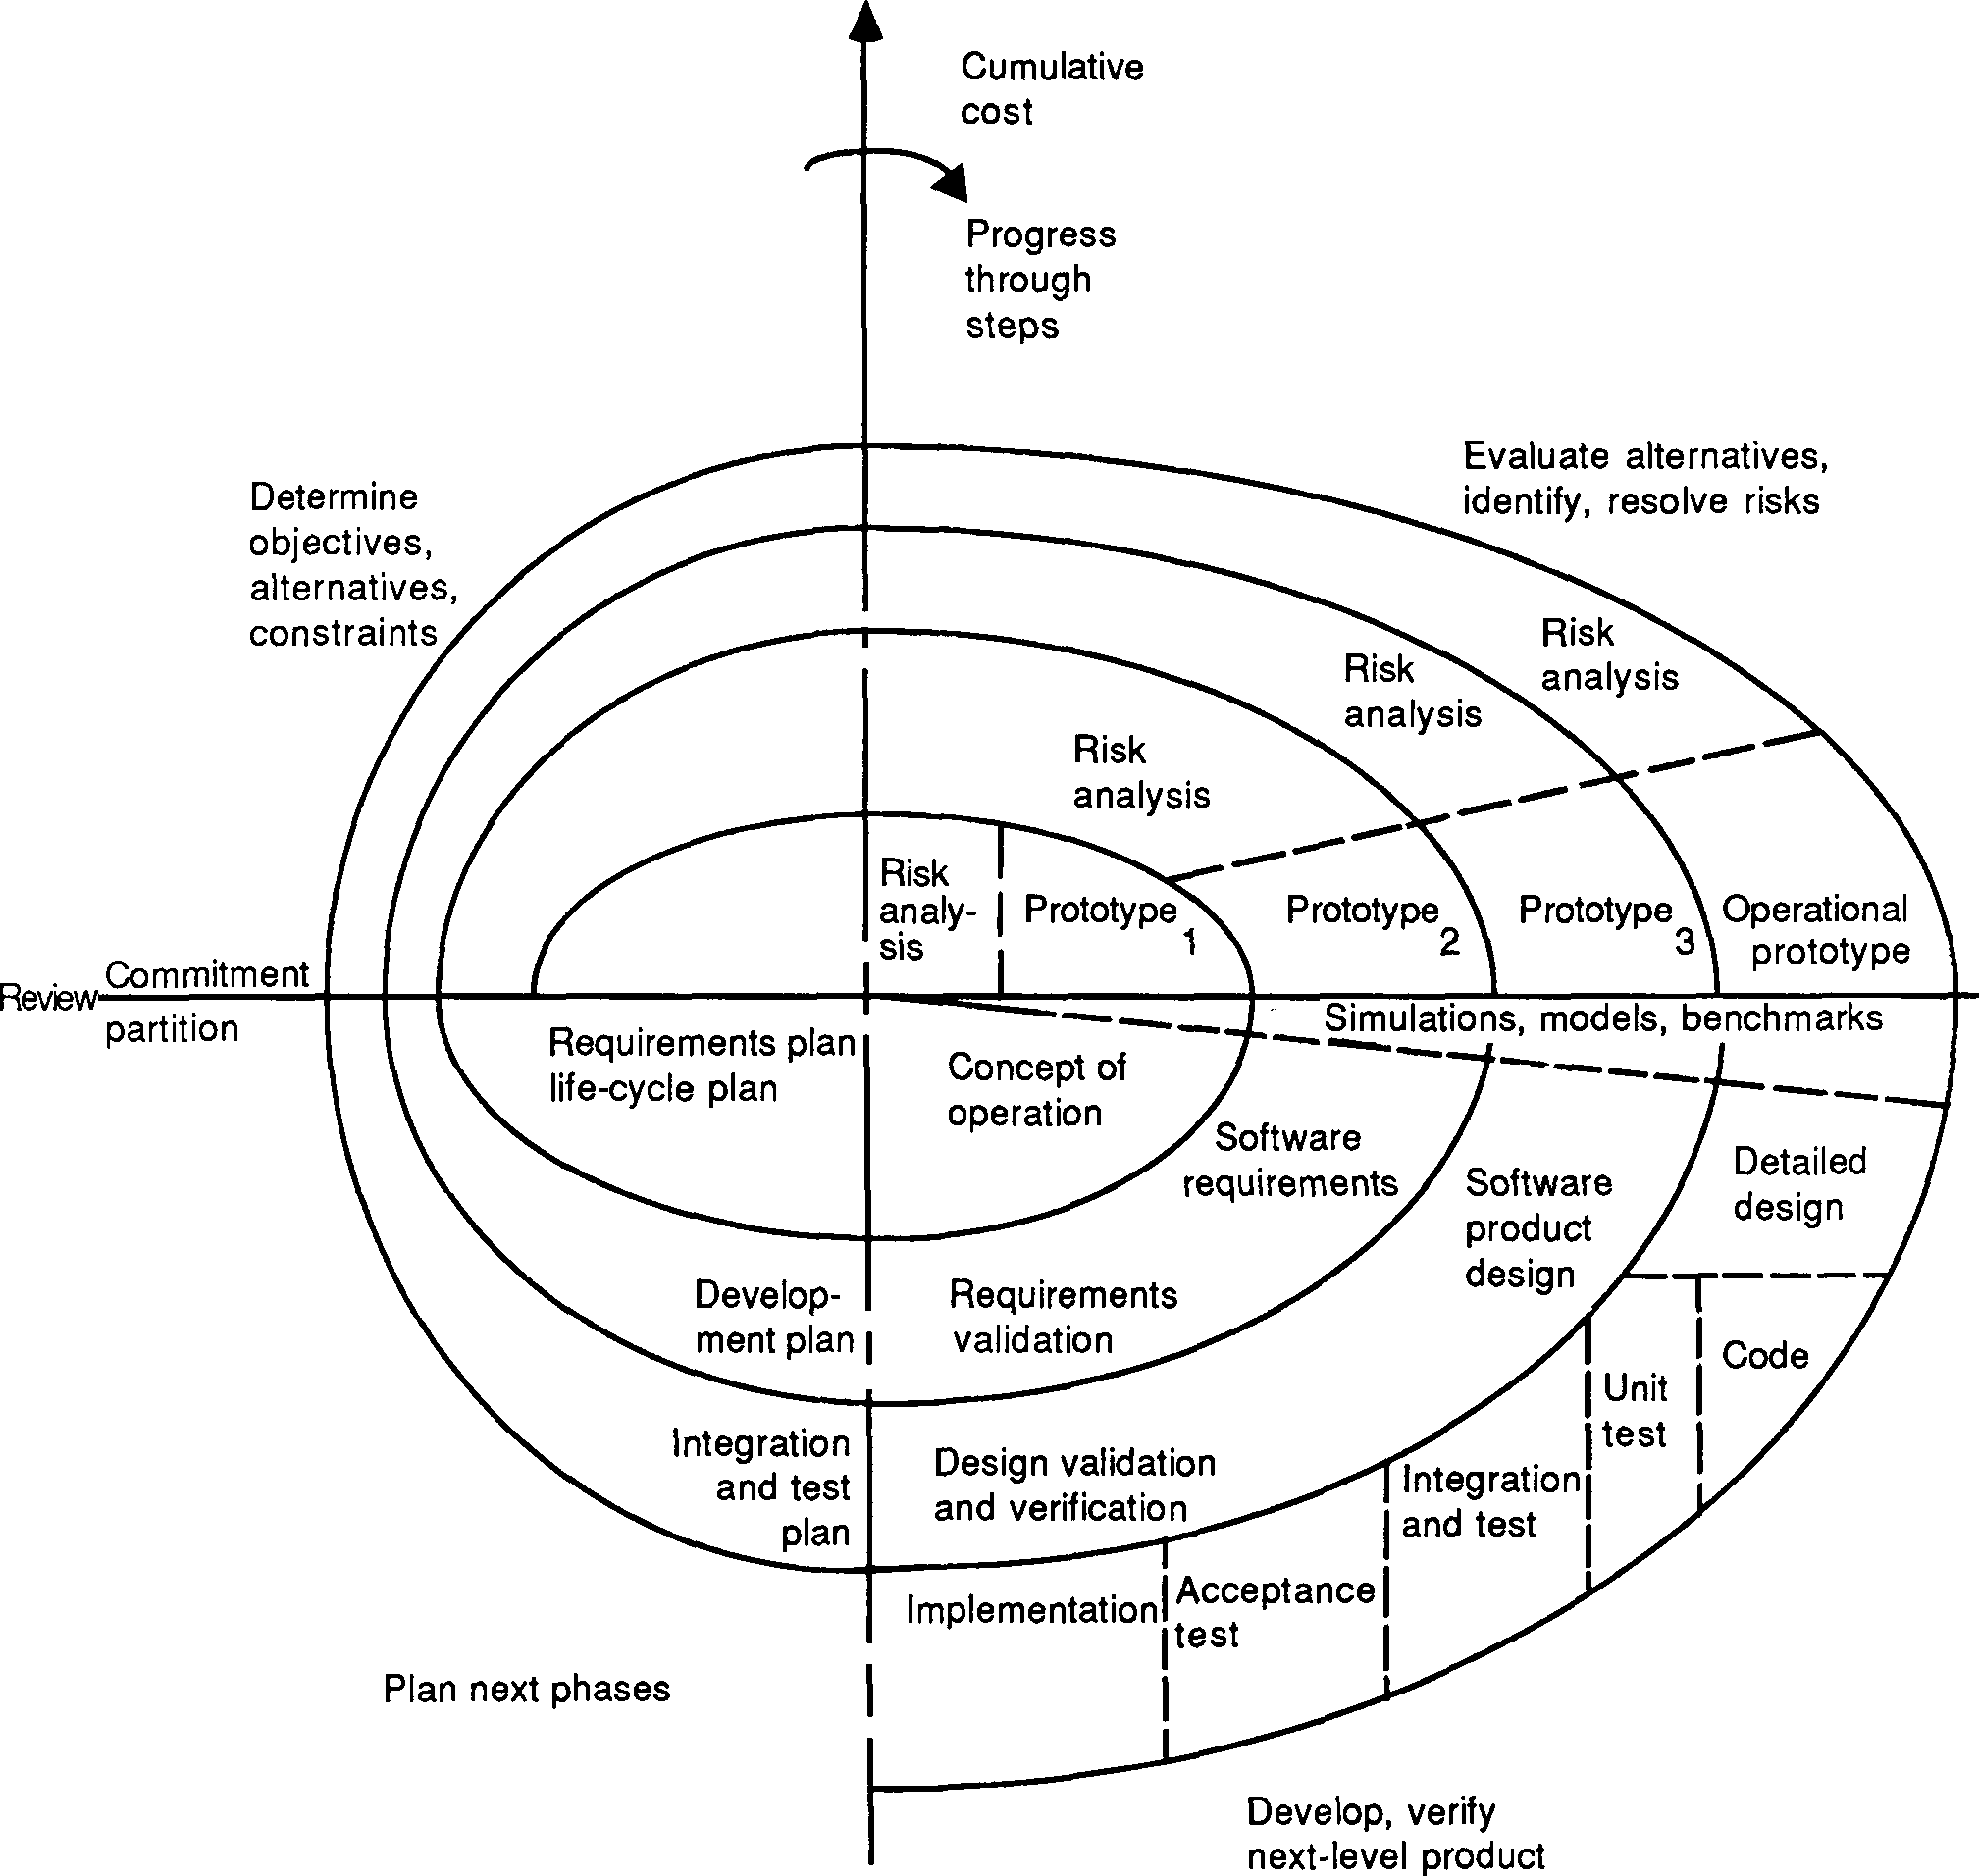
\includegraphics[width=0.4\textwidth]{img/spiral}
%\caption{Spiral model of the software process\cite{59}}\label{fig:spiral}
%\end{figure}

Formal Methods of software development have many different flavours but focus upon proving that a
piece of software satisfies a (formal) specification, typically this specification has a 
mathematical form. Formal Methods are very useful for safety- or mission- critical systems; where
traditional methods would have to rely on large amounts of testing.

It should be pointed out that formal methods do not prove that a program is correct; the methods
only focus on satisfying the specification. If the specification is sufficiently detailed to
ensure the software is correct then it should follow that the formal methods will ensure the
software is correct as well.

Both methods start similarly; gathering requirements for the system. However the Spiral model 
focuses on both requirements and risk analysis whereas Formal Methods these requirements are used
to build an abstract specification.\\

\subsection*{The Vienna Development Model}

This report will focus on the Vienna Development Model (VDM) as the model for a Formal Development
Method, however that are many others with different syntax or structures.

With VDM the two main focuses are on \emph{Data Reification}: the development of abstract data 
types into concrete ones and \emph{Operation Decomposition}: the development of algorithms from
the implicit specification of functions and operations.

The first change that would need to be made is to build this abstract specification based on the
requirements, defining the data types and operations which are needed to complete the system.
Included in these data types are the data type \emph{invariants}; conditions which can relied 
upon to be true.

Along with these data types some theory is also developed, for example if a set within the data
type must have at least one element in it a theory or \emph{lemma} is defined.

With these data types defined the set of operations which need to be performed on them are also
defined. These operations can have both pre- and post- conditions associated with them.




\subsection*{Tool Support}
A number of tools exist to support the conversion of VDM and VDM++ to different languages, 
including Java and C++. VDMTools is one of the leading commercial tools for this area and involves
defining the specification in a text format. VDMTools includes parsers to check both syntax and 
(data) types.

VDMTools also includes ways of performing tests on the specification to ensure that the invariants
and operations are actually defined correctly, these act somewhat similarly to how unit testing
would be performed.


\bibliographystyle{plain}
\bibliography{references}

\end{document}
